\section{Test setup}\label{ssec:test_setup}
To characterise the performance of the linoSPAD under radiation, a test was performed in the cylcotron of the Paul Screrrer Institute (PSI) in Switzerland. The test involved proton radiation beams of both $60\,MeV$ and $10.1\,MeV$. A schematic of the setup is shown in ??. HIER MOET WAT BLAAT IN
.






\begin{figure}[h]
\centering
	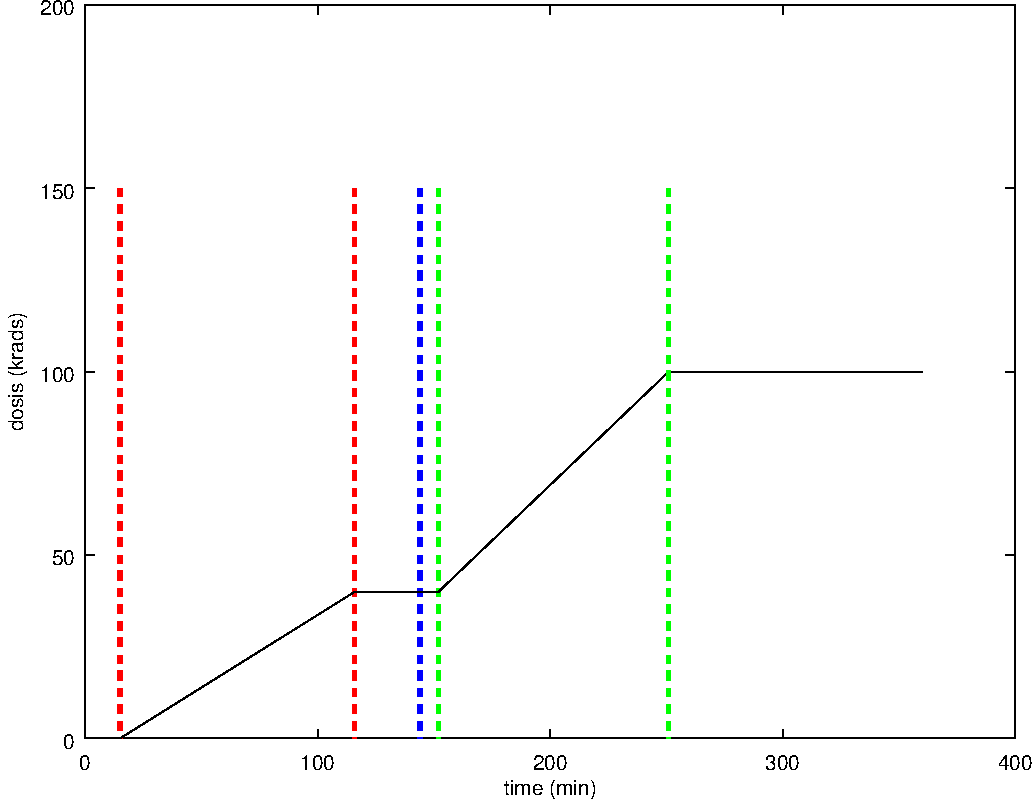
\includegraphics[width=0.6\linewidth]{fig/dosis.pdf}
\caption{The accumulative dose of radiation produces by the proton radiance as a function of time}
\label{fig:dosis}
\end{figure}


